\documentclass{article}
\usepackage{subfigure}
% Language setting
% Replace `english' with e.g. `spanish' to change the document language
\usepackage[english]{babel}

% Set page size and margins
% Replace `letterpaper' with `a4paper' for UK/EU standard size
\usepackage[letterpaper,top=2cm,bottom=2cm,left=3cm,right=3cm,marginparwidth=1.75cm]{geometry}

% Useful packages
\usepackage{amsmath}
\usepackage{graphicx}
\usepackage{float}
\usepackage[colorlinks=true, allcolors=blue]{hyperref}

\title{Suicidal Tendency Among Schizophrenia-Diagnosed Patients}
\author{Haim Lavi, 038712105}

\begin{document}
\maketitle

\begin{abstract}
In this paper, I shall analyze a dataset from Turkey, containing different features on people who are either diagnosed or not diagnosed as having Schizophrenia. Although there is much to study from this dataset about the disease itself, I shall concentrate in Schizophrenia-diagnosed people, and their tendency to attempt to commit suicide. I shall use unsupervised learning methods to find general patterns in the data, and by these patterns I will be able to identify this particular feature (suicide attempt), and I will try to check if it has any statistical relation to other features, or it stands by itself.
\end{abstract}

\section{Introduction}
\subsection{General Explanation}
Schizophrenia is a serious mental illness that affects the patient and disables him or her from performing as a fully capable valid person. The question of why someone has Schizophrenia does not always have a decisive answer, because there are many factors that can cause this situation, genetic and environmental. Research in this field can help find helpful ways to tackle this harsh situation, because, if we find several factors which are statistically observed as common among people who have Schizophrenia, especially if we find the most common ones, then neutralizing some of these factors can help in preventing the abruption of this mental condition. Another major question, which we shall also concentrate in, is, when we have a patient diagnosed with Schizophrenia, what must we consider regarding his or her own personal safety and well-being.
\subsection{This Paper Research}
I have found in Kaggle a dataset containing data collected among people in Turkey. The dataset contains several data features that I would like to divide to three categories:
\begin{enumerate}
    \item Features that are basic to any research on human beings, such as age and gender.
    \item Features that directly correspond to the subject of Schizophrenia, above all is the diagnosis itself (diagnosed / not diagnosed as Schizophrenic), as well as mental and behavioral tests.
    \item Physical / Behavioral / Environmental features, that are suspected or known as factors for Schizophrenia, whether their influence is positive (having more of) or negative (having less of).
\end{enumerate}
\subsection{Main Question}
One major question, regarding people diagnosed as Schizophrenic, is whether they are suicidal or not. The danger of having a person committing suicide can dictate the use of extreme safety measures, such as using heavy drugs or straitjackets. But if we can identify features that distinguish between different people who have Schizophrenia, we can avoid using those measures, and keep them only for people who share features that are highly related to being suicidal. 
For instance, since committing suicide is an act of self-violence, we would expect this to be less common in females than in males, or we would expect this more in younger people rather than the matured age. Also, we can expect this to be more common in people who are addicted to drugs, which usually increase the violent tendencies of the person consuming them.
This question arose directly from the unsupervised data analysis, as shall be explained later.
\section{Methods}
\subsection{Dimensionality Reduction}
I used three methods for the reduction of dimensionality.
\begin{enumerate}
    \item PCA
    \item t-SNE
    \item UMAP
\end{enumerate}

\subsection{Clustering}
I used three methods for clustering.
\begin{enumerate}
    \item K-Means
    \item DBSCAN
    \item Gaussian Mixture
\end{enumerate}

For methods that are given the expected number of clusters, I have iterated over a range of possible numbers, calculating the silhouette score on each iteration, and updating a stored value of the maximum score. While the minimum number of clusters is naturally 2, the maximum number is a matter of guessing.

For the DBSCAN algorithm, which is not based on calculating centroids, I have used the same parameter for calculating the epsilon parameter, by a heuristic function which divides the total area of the set of data points by this increasing factor, yielding a decreasing set of distances, which are used as the epsilon input parameter.

\subsection{Statistical Tests}
For the categorical variables I used the $\chi^2$ test, while for the quantitative variables I used t-test, as shall be explained in the results part. 
\subsection{Remarks}
\begin{enumerate}
    \item Columns to Drop

    Many datasets, including the dataset I was working with, have columns that do not carry any real measurable data, specifically the numeric identifier of the data points, usually it will be the first column. Such columns are not only irrelevant for our analysis, they also add noise, and in order to avoid using them in the process of learning, I added an optional input parameter to the process, telling it to drop specific columns.
    \item Pivot Columns

    As mentioned earlier, our dataset contains features that are directly related to the subject of our study, meaning the diagnosis and the behavioral tests that support it. Thus, it would be useful to identify a target column, in our case the diagnosis, and use it as the pivot of our research, since we want to find ties (or strict differences) between the features that are common among people who are diagnosed as Schizophrenic. For this purpose, I also added an optional input parameter. As a side effect of this, there is the next remark.

    \item Cluster Visualization

    Looking at different examples, there seems to be a tendency to visualize the different clusters using different colors. However, I found that it would be useful for my analysis to visualize the index (cluster label) of each cluster, next to the middle point of the cluster, while using different colors to visualize the value of the target column, as mentioned in the previous remark.

    \item Statistical Tests

    In this paper, and the accompanying code, I use the t-test for quantitative variables, since my choice of optimal clustering goes with the method that yields only two distinguished clusters for the Schizophrenia-diagnosed population. However, while preparing this paper and code I made some statistical tests on a higher number of clusters, using the One-way ANOVA test, and therefore the code basically supports both tests (simply by checking if the number of clusters is 2 or more).

    \item Language Barrier
    
    As specified above, the dataset was collected among people in Turkey. This means that the names of the columns are in Turkish. I have added a small mechanism to tackle this (after trying to add a dynamic call to Google Translate API, with no success), simply by preparing a .csv translation file, and have the code read it and substitute the Turkish names with the English names.
\end{enumerate}
\section{Results}
\subsection{PCA}
I ran the PCA algorithm, as a classic method for reduction of dimensionality from the high dimension to 2 dimensions. Clustering, in this case was quite immediate, since the data is divided in two distinguished bulks, separated along the x-axis (the highest significant dimension), while each bulk keeps the structure of a tight formation, which is more in the shape of an ellipse, with the y-radius measuring longer than the x-radius. For the case of PCA, all the clustering methods that I used yield the same amount of clusters (2), which is the minimum, with relatively high silhouette scores. The advantage of using PCA for this dataset, even though it does not expose a rich structure of the data, is that it shows the general division of the data. Using the Diagnosis column as a pivot, we obtain a clear image of the separation between the two groups of people who are, or are not, diagnosed with Schizophrenia.

\begin{figure}[H]
    \centering
    \subfigure[PCA K-Means]{
        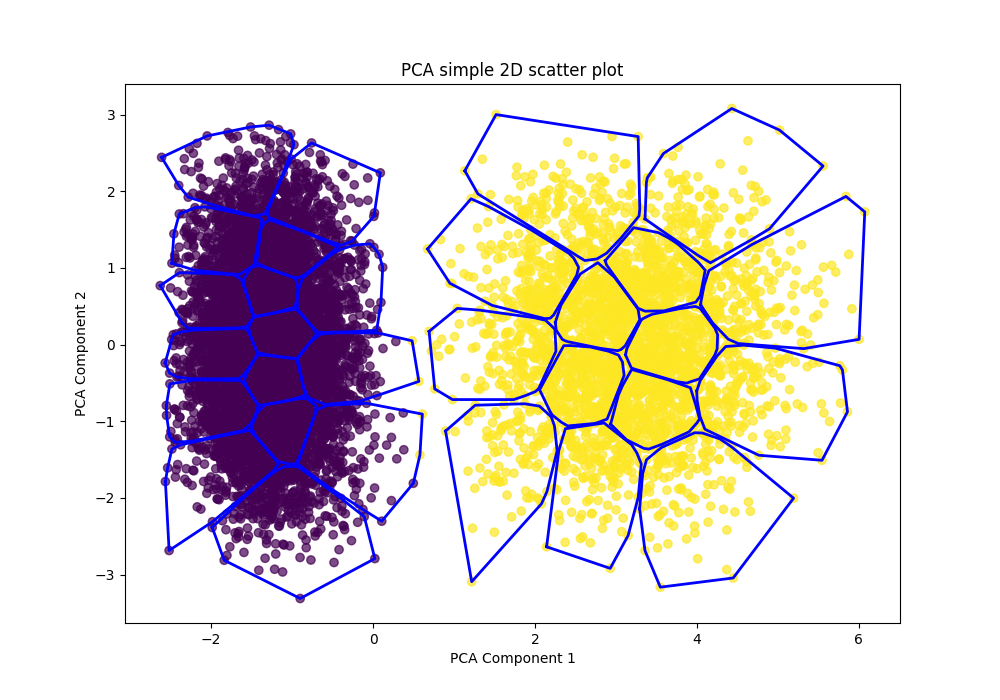
\includegraphics[width=0.3\textwidth]{PCA-KMeans.png}
    }
    \subfigure[PCA DBSCAN]{
        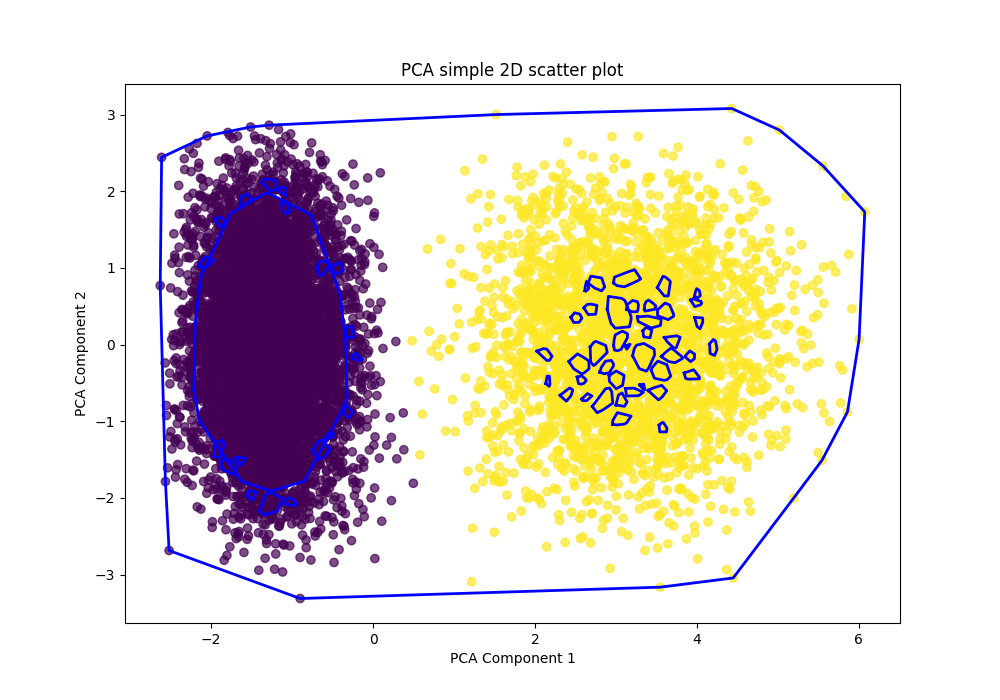
\includegraphics[width=0.3\textwidth]{PCA-DBSCAN.png}
    }
    \subfigure[PCA Gaussian Mixture]{
        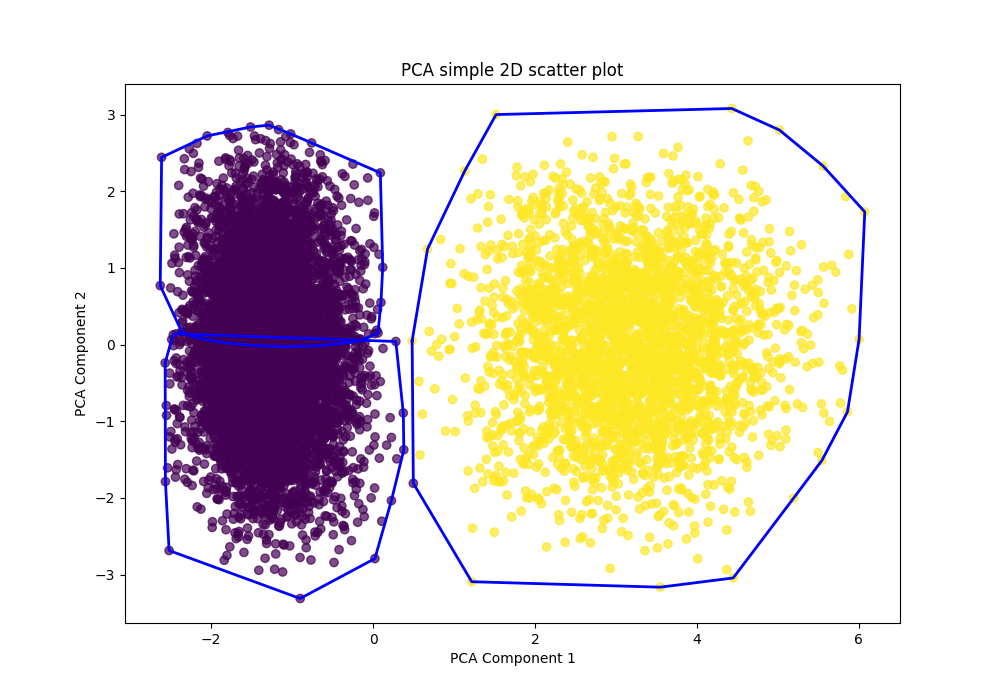
\includegraphics[width=0.3\textwidth]{PCA-GaussianMixture.png}
    }
    \caption{PCA}
\end{figure}

\subsection{t-SNE and UMAP}
Due to the nature of t-SNE and UMAP, and their significant different from the PCA algorithm, I managed to get a better clustering of the data. Using the pivot Diagnosis column, we observe that both populations, the people who are diagnosed with and without Schizophrenia, have inner divisions of their data to separate clusters. Even though the Silhouette scores of the t-SNE clusters are quite lower than those of the clusters that are generated by the UMAP algorithm, they look to the eye as preserving a somewhat similar formation of clusters and neighboring ties (though we have some warping in space between the two sets of clusters, and some of the t-SNE clusters are clearly divided to smaller inner clusters which we do not identify through the algorithm). 
\begin{figure}[H]
    \centering
    \subfigure[t-SNE K-Means]{
        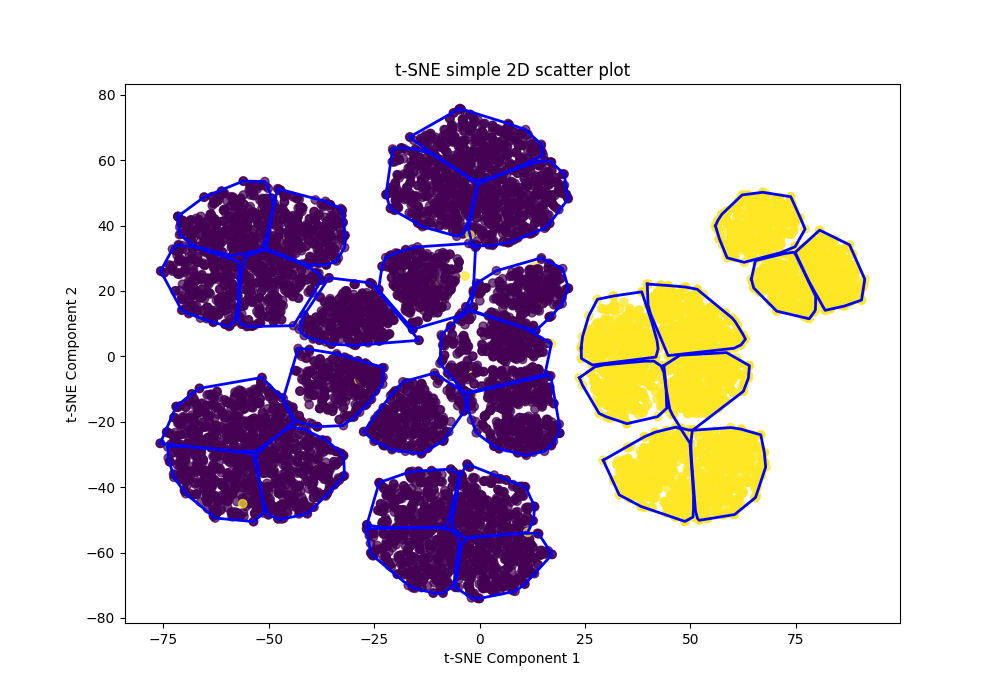
\includegraphics[width=0.3\textwidth]{t-SNE-KMeans.png}
    }
    \subfigure[t-SNE DBSCAN]{
        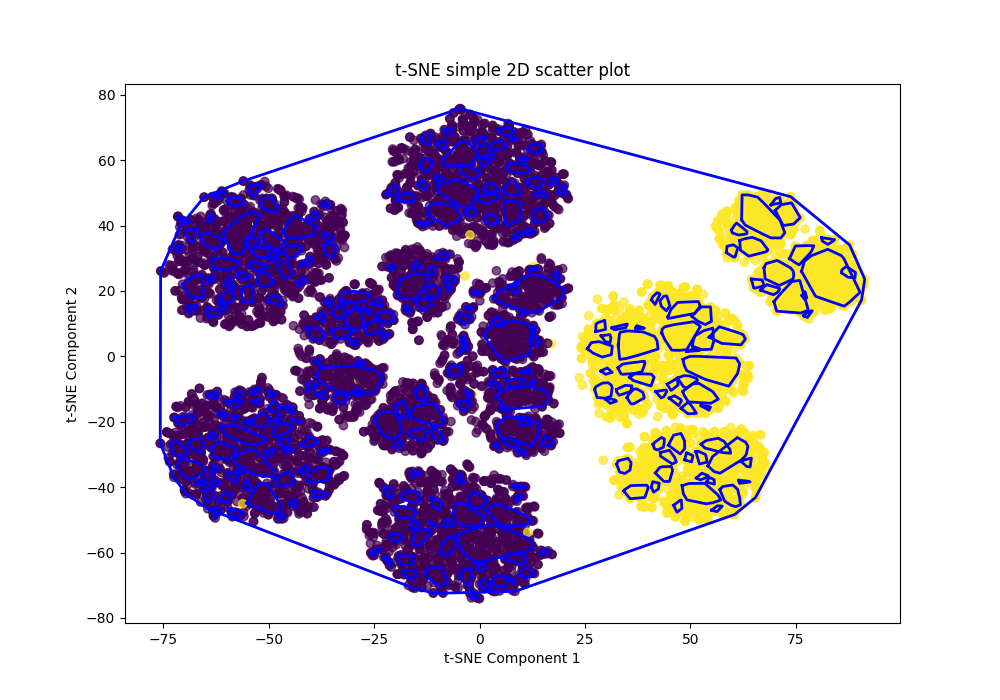
\includegraphics[width=0.3\textwidth]{t-SNE-DBSCAN.png}
    }
    \subfigure[t-SNE Gaussian Mixture]{
        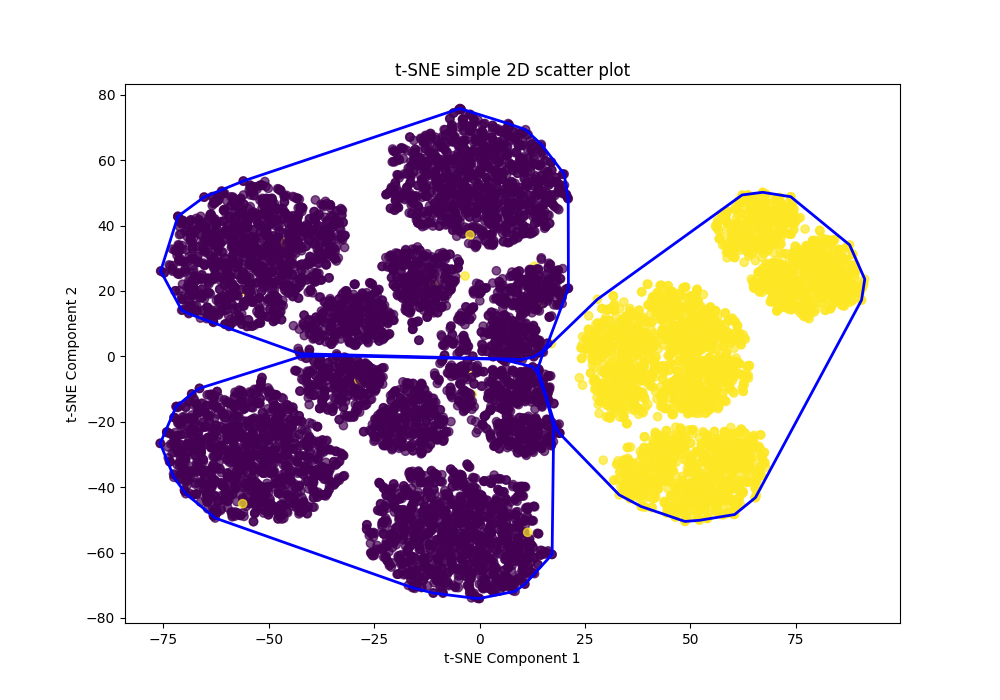
\includegraphics[width=0.3\textwidth]{t-SNE-GaussianMixture.png}
    }
    \caption{t-SNE}
\end{figure}

\begin{figure}[H]
    \centering
    \subfigure[UMAP K-Means]{
        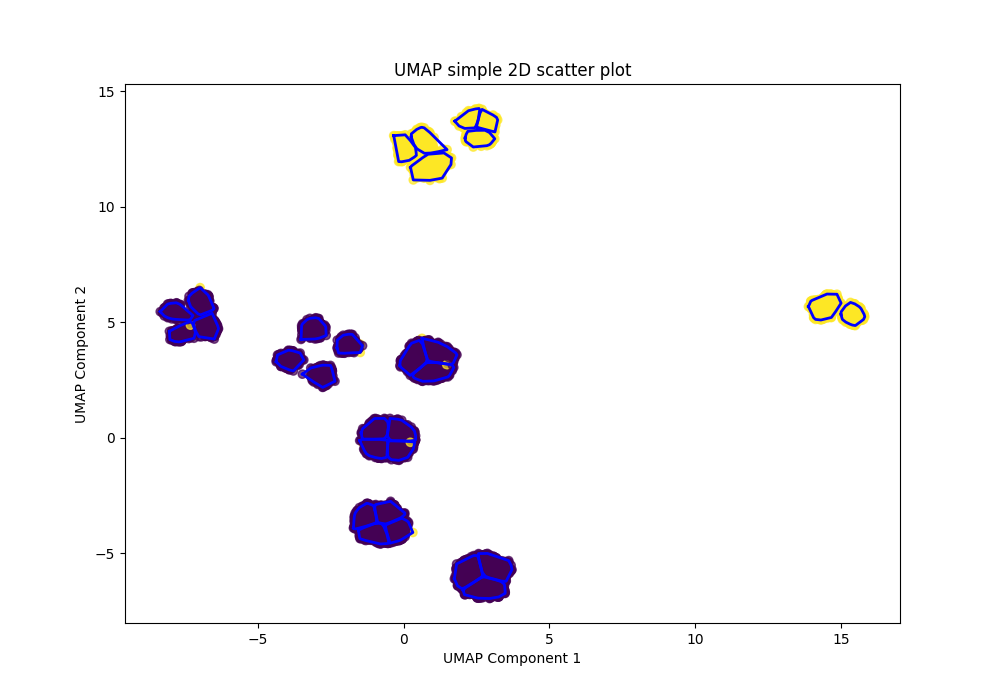
\includegraphics[width=0.3\textwidth]{UMAP-KMeans.png}
    }
    \subfigure[UMAP DBSCAN]{
        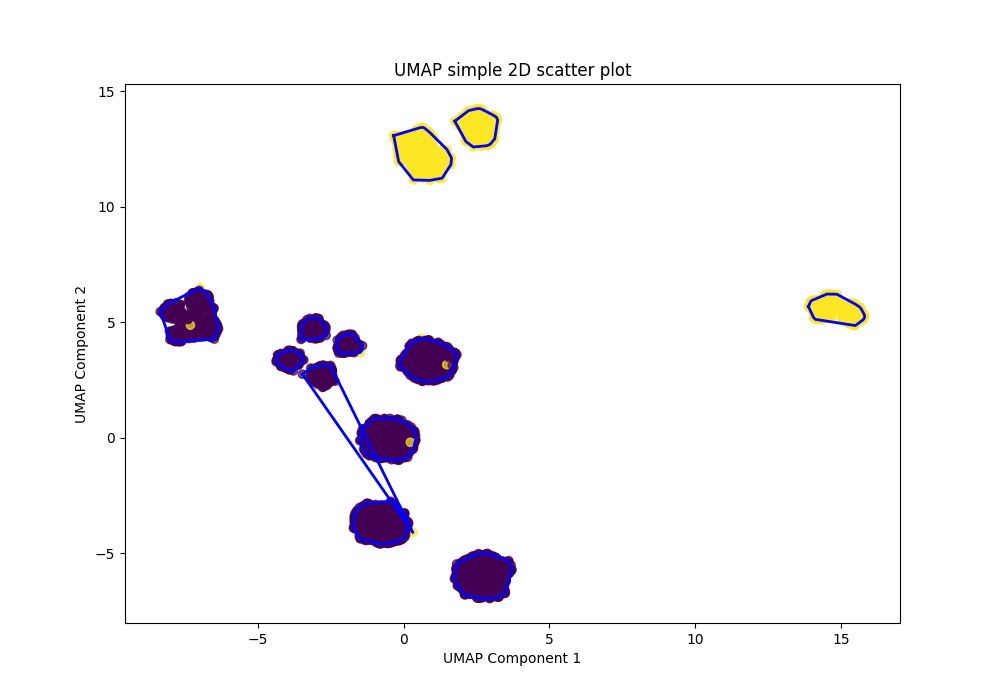
\includegraphics[width=0.3\textwidth]{UMAP-DBSCAN.png}
    }
    \subfigure[UMAP Gaussian Mixture]{
        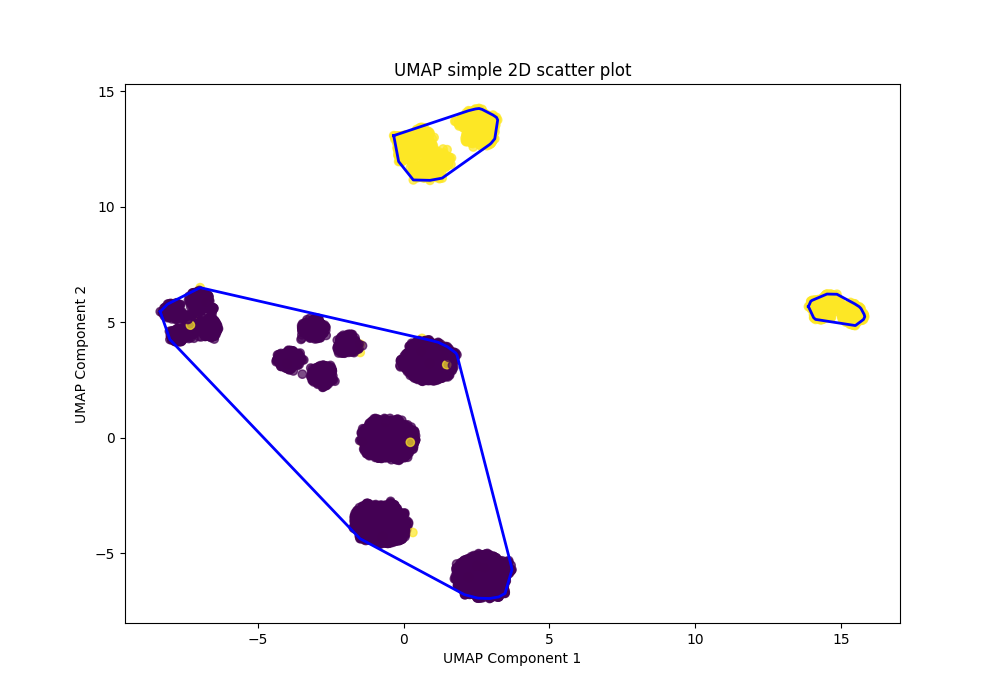
\includegraphics[width=0.3\textwidth]{UMAP-GaussianMixture.png}
    }
    \caption{UMAP}
\end{figure}
The best results achieved by these algorithms are presented in the following table.

\begin{table}[h]
\centering
\begin{tabular}{|l|l|c|c|}
\hline
\textbf{Reducer} & \textbf{Clustering Method} & \textbf{Optimal K} & \textbf{Highest Score} \\
\hline
PCA & KMeans & 2 & 0.7203 \\
PCA & DBSCAN & 2 & 0.7203 \\
PCA & GaussianMixture & 2 & 0.7203 \\
t-SNE & KMeans & 9 & 0.5343 \\
t-SNE & DBSCAN & 9 & 0.5343 \\
t-SNE & GaussianMixture & 9 & 0.5338 \\
UMAP & KMeans & 8 & 0.8477 \\
UMAP & DBSCAN & 8 & 0.8477 \\
UMAP & GaussianMixture & 8 & 0.8477 \\
\hline
\end{tabular}
\caption{Comparison of Dimensionality Reduction and Clustering Methods}
\label{tab:reduction_clustering_comparison}
\end{table}
\subsection{Optimal Results}
As can be seen in the results table, the optimal method, according to the Silhouette score, is UMAP, with either of the three used clustering methods, while it may seem to the eye that we get slightly better results with a different method. For instance, we get a finer division of the dataset to clusters using t-SNE with Gaussian Mixture, as can be seen in the table and from the figures above. This emphasizes the fact that unsupervised learning can be analyzed in different ways, and different patterns and ties can be found with each of them. For this paper, I prefer to stick with the division which is considered the optimal by the Silhouette score.
For an easier analysis of the data, we can display the best results in a heatmap, where we display the means of all the features, for each cluster, and observe the similarities and differences between the clusters.

\begin{figure}[H]
    \centering
    \subfigure[heatmap for UMAP]{
        \includegraphics[width=1\textwidth]{UMAP-KMeans-heatmap.png}
    }
\end{figure}

We can clearly observe from the heatmap that the subject-oriented columns (Diagnosis and the three behavioral scores) form a strong distinction between the two populations, the diagnosed people, and the people who are not diagnosed. This can lead us to working on different questions. What got my eye was the difference between the two clusters of diagnosed people, namely 1 and 4 (since the scores for all the clusters of the UMAP algorithm are the same, we randomly pick the K-Means clustering, so we can see the indexed clusters in the UMAP K-Means image above).
As it appears, the only significant difference between these two clusters is in the suicide attempt column, which says, if we can prove it statistically, that \textbf{other features, existing in this dataset, do not influence the suicidal tendency of the diagnosed person}, which can lead to the harsh conclusion, that Schizophrenic people may attempt to commit suicide, or avoid this, regardless of other parameters, such as the group in population they belong to (male/female, young/old etc.), or their environmental and genetic factors (family history, stress factors, social support etc.), thus being a substantial challenge for the mental health teams taking care of them. 
Using the $\chi^2$ for categorical variables (which are the majority of the variables in this dataset) and t-test for variables such as gender, durasion of disease etc., we do establish the above observation through statistical tests, as shown in the following table.
\begin{table}[ht]
\centering
\begin{tabular}{|l|c|}
\hline
\textbf{Column} & \textbf{p-value} \\
\hline
Age & 0.3404 \\
Gender & 0.6779 \\
Education Level & 0.1944 \\
Marital Status & 0.3908 \\
Occupation & 0.1858 \\
Income Level & 0.7828 \\
Place of Residence & 0.3524 \\
Substance Use & 0.8901 \\
Social Support & 0.1099 \\
Stress Factors & 0.7110 \\
Family History of Schizophrenia & 0.8858 \\
Number of Hospitalizations & 0.6519 \\
Disease Duration & 0.0761 \\
\hline
\end{tabular}
\caption{Table of Columns and p-values}
\end{table}
Taking $0.05$ as the magic value for $p$ in statistical tests, we can see that none of our columns $p$-values has managed to pass the test, that is to say, if $H_0$ is that $\mu_0[\text{column}]=\mu_1[\text{column}]$, where $\mu_0[\text{column}]$ is the mean of the particular column among patients who did not make an attempt to commit suicide, and $\mu_1[\text{column}]$ is the mean among patients who did make an attempt, and $H_a$ is that $\mu_0[\text{column}]\neq\mu_1[\text{column}]$, then it is safe to say that $H_0$ holds for all cases. However, it would be wise to pay attention to relatively small values, particularly values that are rather close to $0.05$, such as the Disease Duration column.

\section{Discussion}
I have shown that the suicidal tendency among the Schizophrenia-diagnosed people in this dataset seems to stand by itself, and is not significantly affected by most other features of the patients. While the wide subject of Schizophrenia, and mental diseases in in general, has almost no limit to the amount of data that can be collected and studies, I would like to concentrate, for this part as well, in the specific subject of suicidal tendency, and suggest a few more features and tests that can be made, in order to both predict, and to avoid, the possible attempt of a Schizophrenic person to commit suicide.
\begin{enumerate}
    \item Religion

    I would suggest any research team in this field to ask also about the level of religious tendency among people who participate in this research (Atheist/Secular/Traditional/Religious/Ultra-Religious etc.), because religion gives a meaning and purpose in life to its believers, and also because most known religions consider suicide a sin.

    \item Sounds

    I could recommend also asking about the patients reactions to different sounds (silence/sounds of the nature/soft music/loud music/comedy skits/news broadcasts etc.), because this can also serve as a positive or negative factor in the way a schizophrenic person feels and behaves. The same goes to sights, like on TV and other digital media

    \item Nutrition

    Another feature that should be documented is the nutrition habits of the people who are diagnosed, or not diagnosed, as Schizophrenic, since it may have influence both on the disease itself, and on the tendency of someone to commit suicide.
\end{enumerate}

There are many other factors that can influence this condition, and all should be studied, for the benefit of the population, but I only stated a few of them which I find particularly influencing.

\section{Links}
git repository: \url{https://github.com/HaimL76/unsupervised.git}\newline
overleaf project: \url{https://www.overleaf.com/read/dyrnjnxdkbkf#908474}\newline
executable file: \url{https://drive.google.com/file/d/1J-hOjCndZ0Q3PCy5jHOU1jL5xxLNBAiU/view?usp=sharing}

\begin{thebibliography}{2}
\bibitem{PCA1}
https://www.linkedin.com/pulse/principal-component-analysis-pca-made-easy-mario-la-rocca
\bibitem{Silhouette1}
https://www.analyticsvidhya.com/blog/2021/05/k-mean-getting-the-optimal-number-of-clusters/
\bibitem{DBSCAN1}
https://www.geeksforgeeks.org/dbscan-clustering-in-ml-density-based-clustering/
\bibitem{GaussianMixture1}
https://www.geeksforgeeks.org/gaussian-mixture-model/
\end{thebibliography}
\end{document}